\documentclass[a4paper,11pt]{article}

\usepackage{etoolbox}
\usepackage{fancyvrb}
\usepackage[T1]{fontenc}
\usepackage{graphicx}
%\usepackage{import}
\usepackage{listings}
%\usepackage{minted}
\usepackage{url}

\usepackage[
	% Prevent hyperlinks from getting an ugly border
    hidelinks,
    % Set proper PDF metadata
    pdftex,
    pdfauthor={Your Name},
    pdftitle={Thesis Title},
    pdfsubject={PDF Subject},
    pdfkeywords={keyword1, keyword2, keyword3}
]{hyperref}

% Don't display "References" when rendering the bibliography
\patchcmd{\thebibliography}{\section*{\refname}}{}{}{}

% Use appropriate font size for line numbers in listings
\renewcommand{\theFancyVerbLine}{{\small\arabic{FancyVerbLine}}}

\lstset{basicstyle=\ttfamily}
\newcommand{\code}[1]{\texttt{#1}}

\setlength{\footnotesep}{0.4cm}
\setlength{\skip\footins}{0.5cm}

\def\doctype{Bachelor's Thesis in Computer Science}
\def\title{The Title \\ of your Thesis}
\def\author{Your Name}
\def\date{Submission Date}

\begin{document}

\thispagestyle{empty}

\def\bcorcor{0.15cm}
\addtolength{\hoffset}{\bcorcor}

\thispagestyle{empty}

\vspace{4cm}

\begin{center}

  \begin{figure}[h]
    \centering
    
\includegraphics[width=4cm\textwidth]{sections/_meta/hsba-logo}
  \end{figure}
  
  \vspace{5mm}
  
  \huge DEPARTMENT OF COMPUTER SCIENCE\\
  
  \vspace{0.5cm}
  
  \large HAMBURG SCHOOL OF BUSINESS ADMINISTRATION
  
  \vspace{1mm}
\end{center}

\vspace{15mm}

\begin{center}
  {\Large \doctype}

  \vspace{10mm}

  \setlength\lineskip{8pt}
  {\LARGE \bf \title}\\%[3ex]

  \vspace{15mm}

  {\LARGE \author}

  \vspace{10mm}
  
  \begin{figure}[h!]
    \centering
    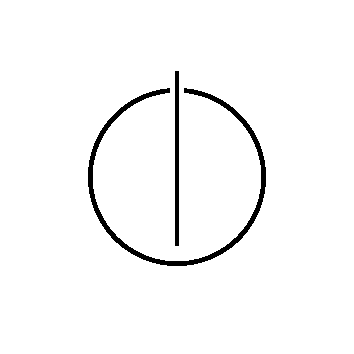
\includegraphics[width=4cm]{sections/_meta/informat.png}
  \end{figure}
\end{center}

\thispagestyle{empty}

\def\bcorcor{0.15cm}
\addtolength{\hoffset}{\bcorcor}

\thispagestyle{empty}

\vspace{4cm}

\begin{center}

  \begin{figure}[h]
    \centering
    
\includegraphics[width=4cm\textwidth]{sections/_meta/hsba-logo}
  \end{figure}

  \vspace{5mm}
  
  \huge DEPARTMENT OF COMPUTER SCIENCE\\
  
  \vspace{0.5cm}
  
  \large HAMBURG SCHOOL OF BUSINESS ADMINISTRATION\\
  
  \vspace{1mm}
\end{center}

\vspace{15mm}

\begin{center}
  {\Large \doctype}

  \vspace{20mm}

  \setlength\lineskip{8pt}
  {\LARGE \bf \title}\\%[3ex]

  \vspace{10mm}

  {\LARGE \germantitle}
\end{center}

\vfill

\renewcommand{\arraystretch}{0.7}

\begin{center}
\begin{tabular}{l@{\hskip 1cm}l}
  {\Large \bf Author:} & {\Large Your Name} \\\\
  {\Large \bf Supervisor:} & {\Large Name of your Supervisor} \\\\
  {\Large \bf Advisor:} & {\Large Name of your Advisor} \\\\
  {\Large \bf Submission date:} & {\Large Submission Date}
\end{tabular}
\end{center}

\thispagestyle{empty}

\vspace*{\fill}
\begin{flushright}
\noindent \textit{I confirm that this bachelor's thesis is my own work \\ and I have documented all sources and material used.\\[\baselineskip]}
City, Submission Date \\[3.5\baselineskip]
\underline{\hspace{6.5cm}}
\end{flushright}


\newpage
\thispagestyle{empty}
\null

\newpage
\thispagestyle{empty}
\section*{Abstract}

 Your abstract goes here

\newpage
\pagestyle{empty}
\tableofcontents

\newpage
\pagestyle{plain}
\setcounter{page}{1}

% Include sections here
% \section{Introduction}

You can write an introduction here and add different sections like...

\subsection{Research Question}
\label{sec:motivation}

Write something about the research question...
\subsection{Motivation}
\label{sec:motivation}

Write something about the motivation...


\subsection{This Thesis' Structure}
\label{sec:motivation}

Write something about the structure of your thesis...


% Include refereces here
\section{References}
\bibliography{references}
\bibliographystyle{plain}

% Include appendix here
% \section{Appendix A}
\label{sec:appendix}

You can include your appendix here.

% To add the first section to your appendix create a new .tex file and include it like so:
% \subsubsection{Subsection 1}

% To add another section to your appendix create a new .tex file and include it like so:
% \newpage
% \subsubsection{Subsection 2}


\end{document}
